\documentclass{beamer}
\usepackage[utf8]{inputenc}

\usetheme{Madrid}
\usecolortheme{default}
\useinnertheme{circles}

\definecolor{Logo1}{rgb}{0.208, 0.2865, 0.373}
\definecolor{Logo2}{rgb}{0.000, 0.674, 0.863}

\setbeamercolor*{palette primary}{bg=Logo1, fg=white}
\setbeamercolor*{palette secondary}{bg=Logo2, fg=white}
\setbeamercolor*{palette tertiary}{bg=white, fg=Logo1}
\setbeamercolor*{palette quaternary}{bg=Logo1,fg=white}
\setbeamercolor{structure}{fg=Logo1} % itemize, enumerate, etc
\setbeamercolor{section in toc}{fg=Logo1} % TOC sections

\usepackage{graphicx,animate}
%------------------------------------------------------------
%This block of code defines the information to appear in the
%Title page
\title[Linear Algebra] %optional
{Orthogonality, and Something Interesting...}

\subtitle{Lecture 7}

\author[11910803@mail.sustech.edu.cn] % (optional)
{
    Zhang Ce
}

\institute[] % (optional)
{
    Department of Electrical and Electronic Engineering\\
    Southern University of Science and Technology
}

\date[2021.11.9] % (optional)
{2021.11.9}


%End of title page configuration block
%------------------------------------------------------------



%------------------------------------------------------------
%The next block of commands puts the table of contents at the
%beginning of each section and highlights the current section:

\AtBeginSection[]
{
\begin{frame}
    \frametitle{Table of Contents}
    \tableofcontents[currentsection]
\end{frame}
}
%------------------------------------------------------------


\begin{document}

%The next statement creates the title page.
\frame{\titlepage}


%---------------------------------------------------------
%This block of code is for the table of contents after
%the title page
\begin{frame}
\frametitle{Table of Contents}
\tableofcontents
\end{frame}
%---------------------------------------------------------
\section{Orthogonal Vectors and Subspaces}
\begin{frame}{Inner Product (Dot Product)}
Actually, you have learnt that in your senior high school...

\vspace{3pt}
If I give you 2 vectors $\left[ \begin{array}{c}
	1\\
	2\\
\end{array} \right] ,\left[ \begin{array}{c}
	3\\
	1\\
\end{array} \right]$, how to compute its inner products?

\begin{equation*}
    \left[ \begin{array}{c}
        1\\
        2\\
    \end{array} \right] \cdot \left[ \begin{array}{c}
        3\\
        1\\
    \end{array} \right] =1\times 3+2\times 1=5
\end{equation*}

Recall matrix multiplications, which rule for matrix multiplication is similar to this?

\begin{equation*}
    \left[ \begin{matrix}
        1&		2\\
    \end{matrix} \right] \left[ \begin{array}{c}
        3\\
        1\\
    \end{array} \right] =3+2=5
\end{equation*}

Therefore, for 2 vectors $u$ and $v$, the inner product is $u^Tv$.

\vspace{3pt}
Take a deeper look, the result $5$ shows us... Think in geometrical way!
\end{frame}

\begin{frame}{Inner Product (Dot Product)}
\begin{figure}
    \centering
    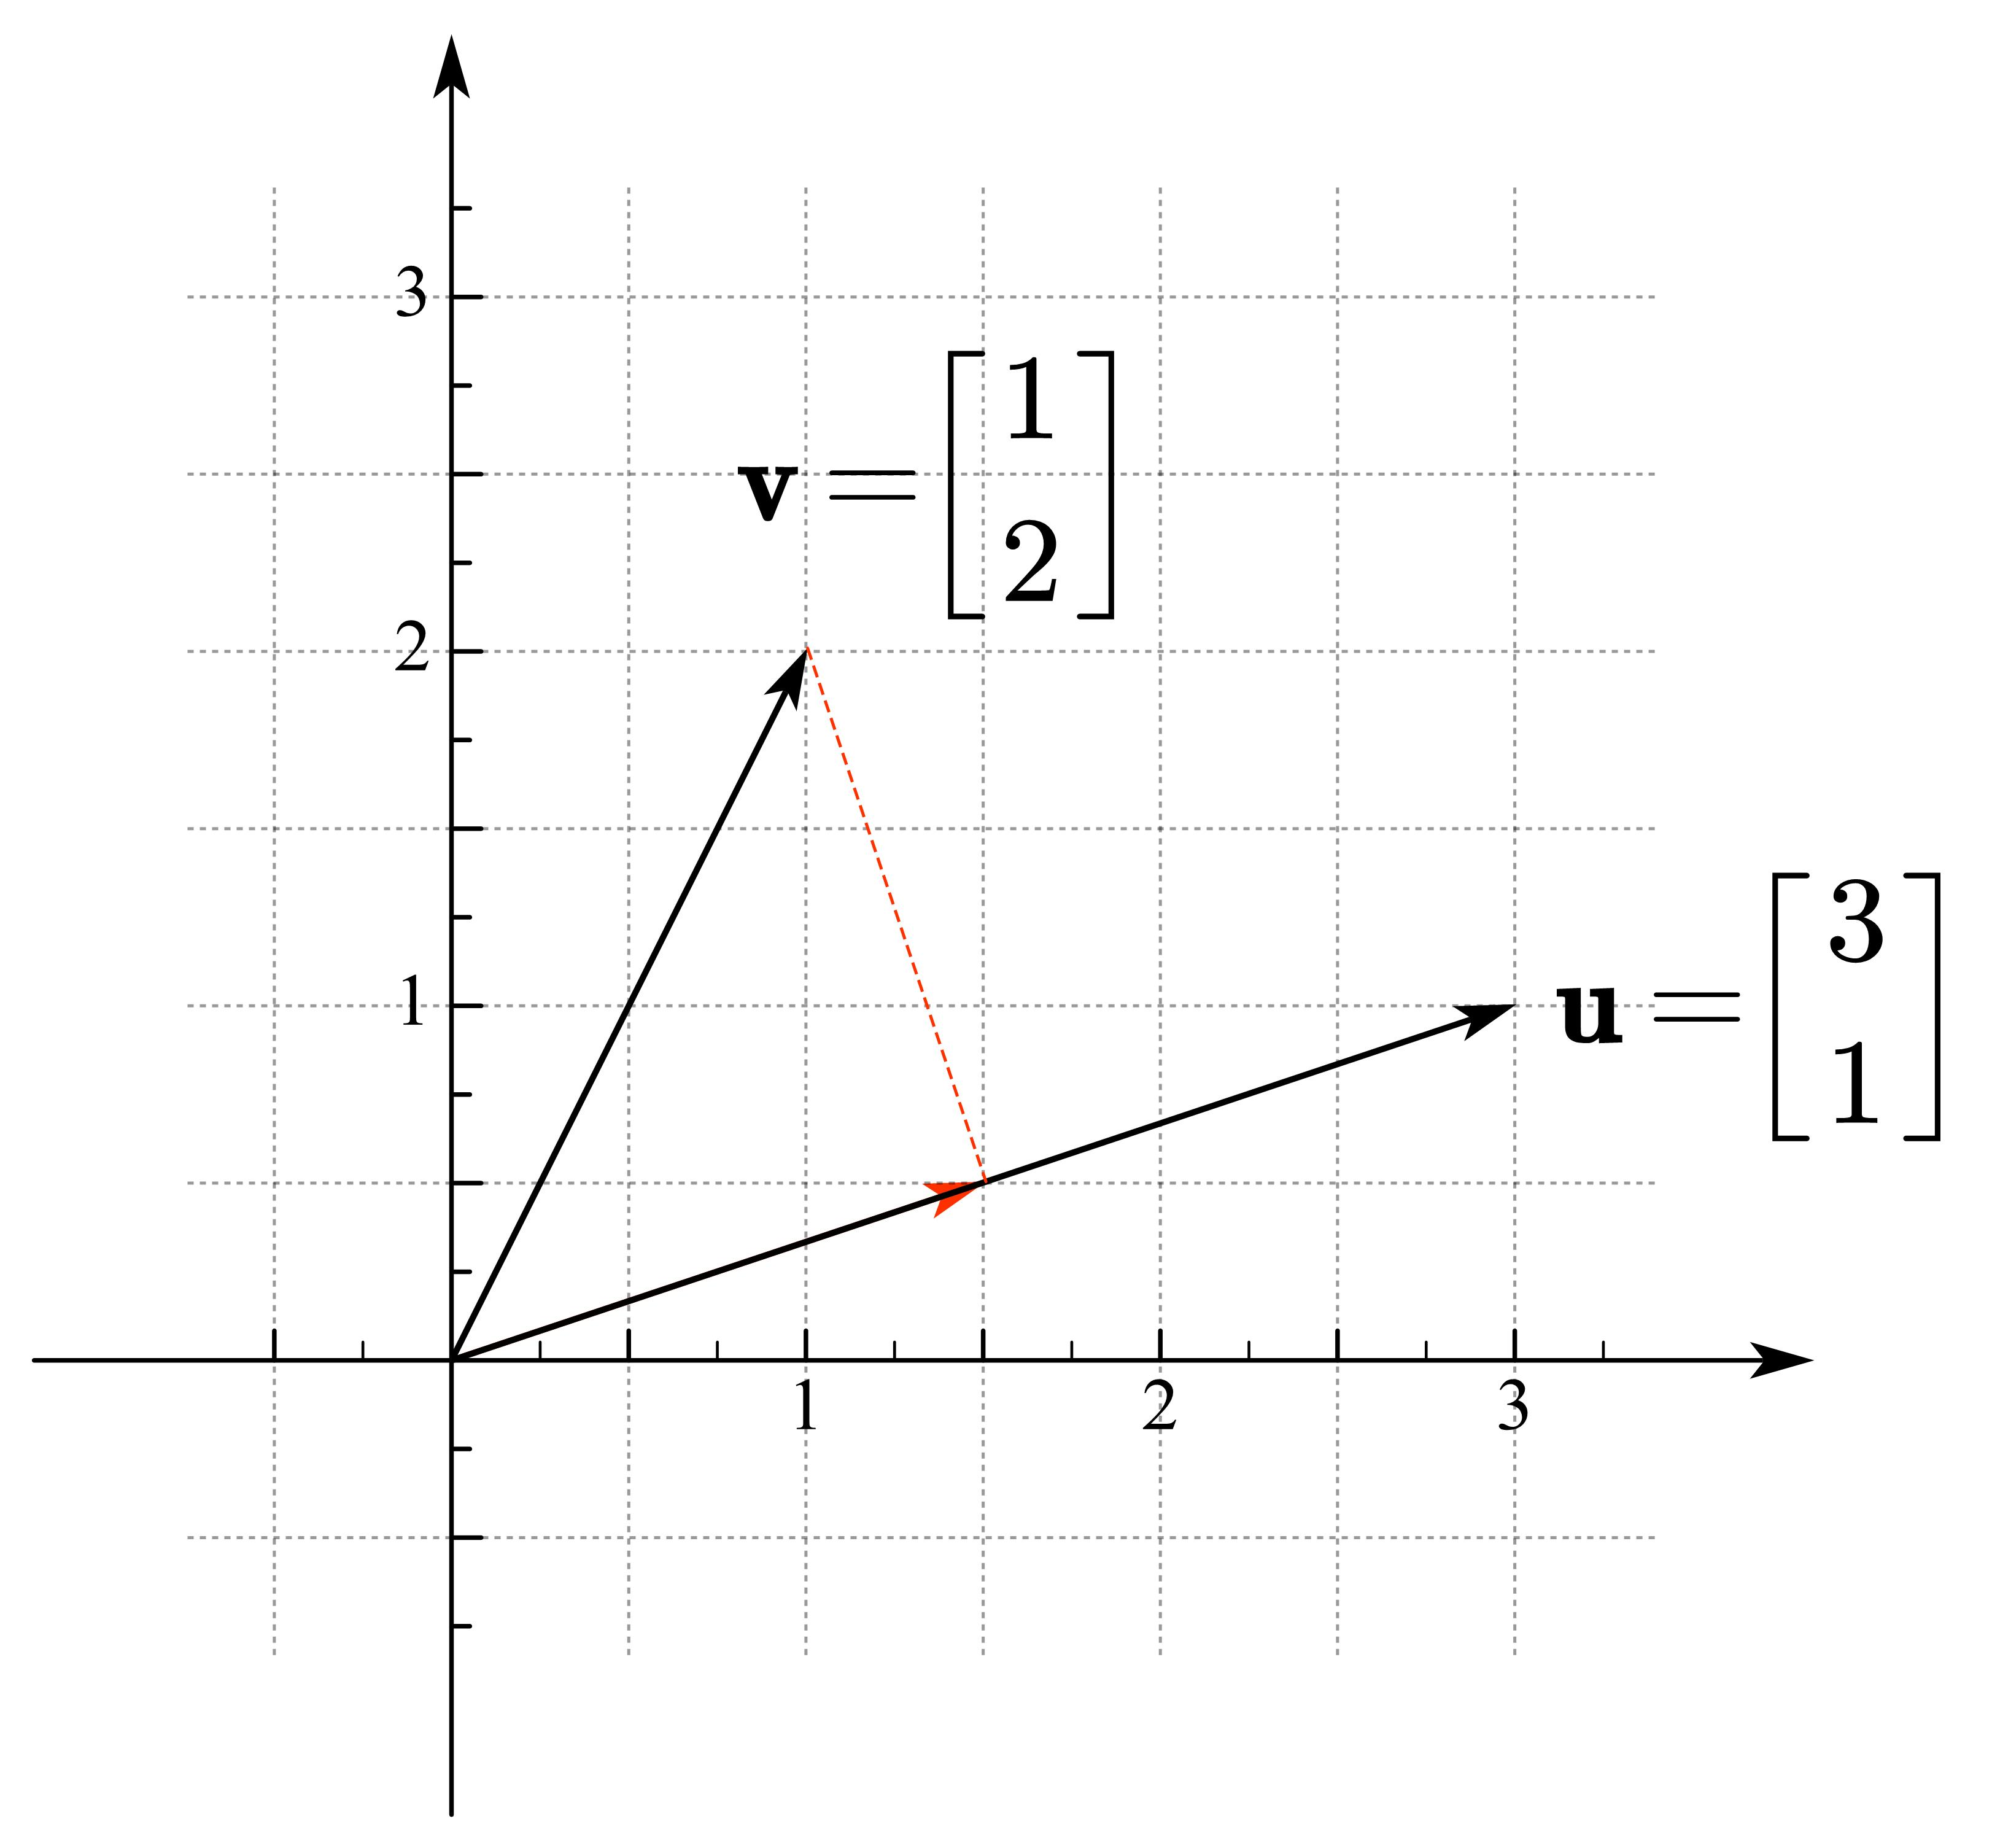
\includegraphics[width=0.47\textwidth]{ip.jpg}
\end{figure}

In my perspective, there inner product reflects their relevance. If the inner product can take the maximum or minimum value, then the vectors are dependent. While if the inner product is greater than zero, they point to the same direction, if it equals to zero, they have nothing to do with each other (perpendicular).
\end{frame}

\begin{frame}{Orthogonal Vectors and Subspaces}
Which value of inner product can let you realize that the vectors are perpendicular (\alert{orthogonal})?
\begin{equation*}
    u^Tv=0
\end{equation*}

Then we can further extend this definition to subspaces, if all the vectors in subspace $A$ are orthogonal to all the vectors in subspace $B$, then suspaces $A$ and $B$ are orthogonal.

\vspace{3pt}
One good question to ask: Is the blackboard plane perpendicular to the ground? But are they orthogonal?

\vspace{3pt}
Well, two orthogonal subspaces can only have the origin in common, and that is from the restriction of subspaces!
\end{frame}

\section{Projections onto Lines}
\begin{frame}{Projections}
Let's start from geometrical view. We want to find projection $\mathbf{p}$.
\begin{figure}
    \centering
    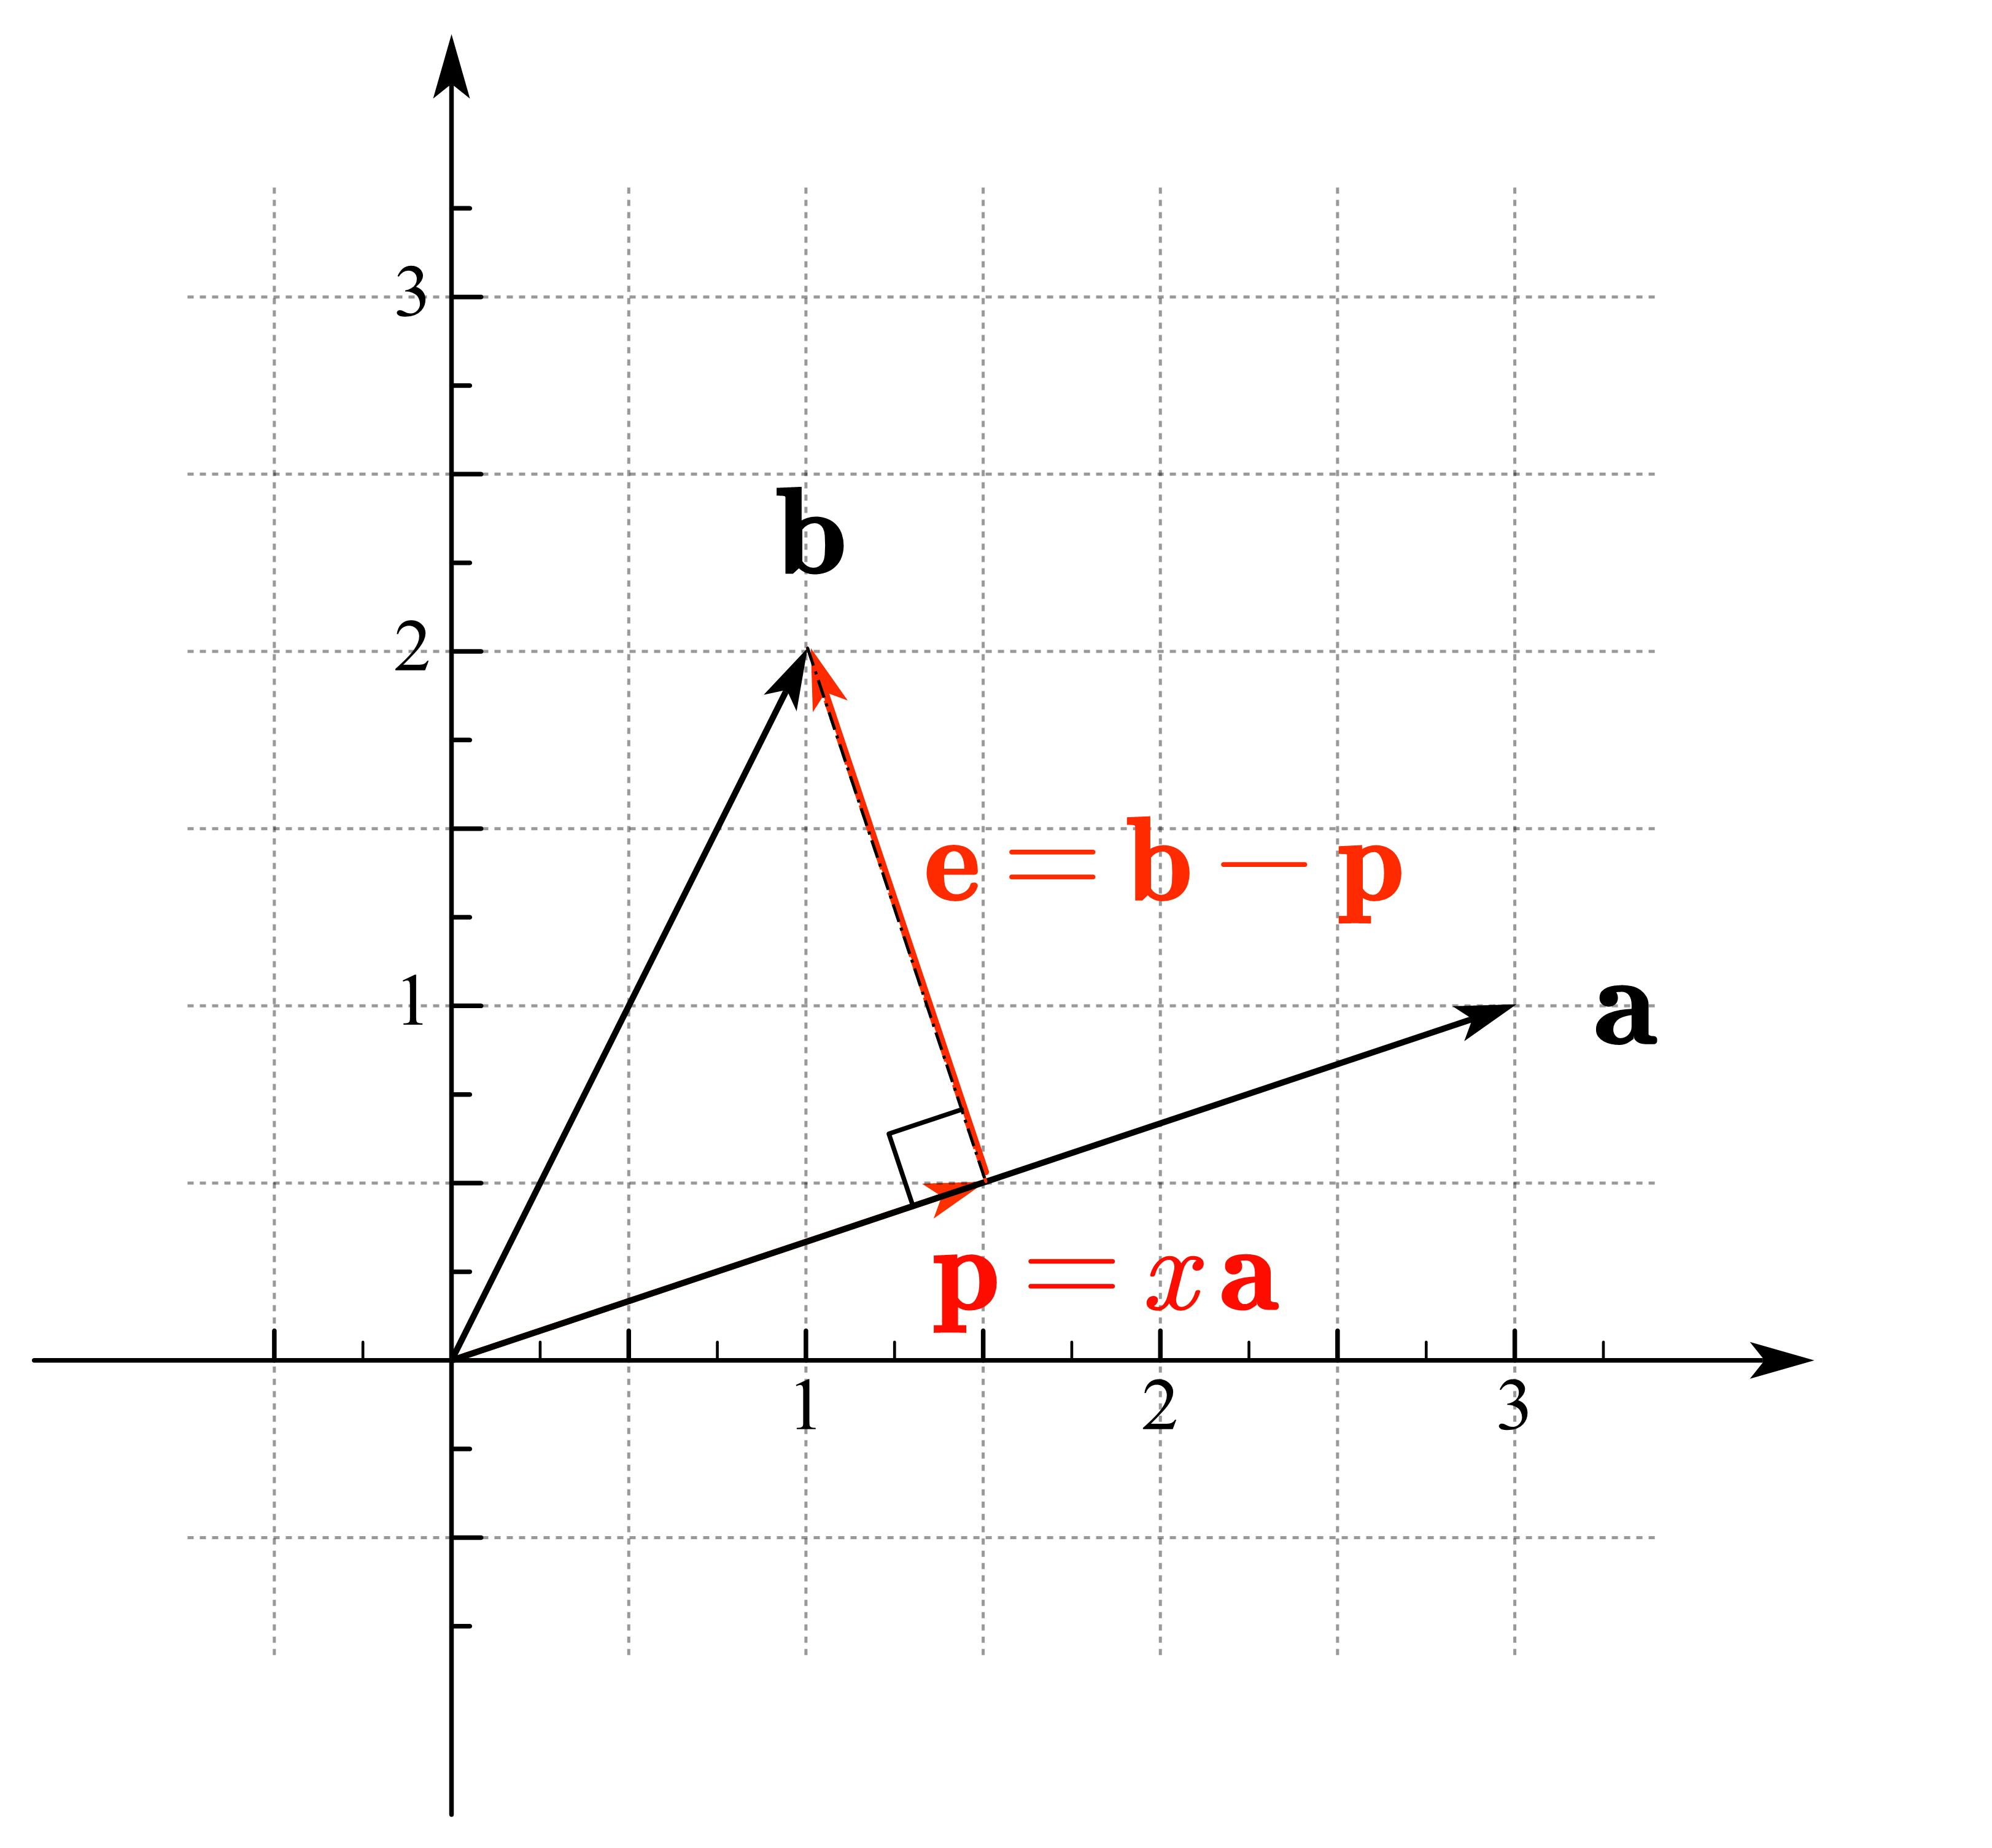
\includegraphics[width=0.45\textwidth]{projection.jpg}
\end{figure}

What can we get from that 90 degrees? Can we get an expression of $\mathbf{p}$?
\begin{equation*}
    \mathbf{a}^T\mathbf{e}=\mathbf{a}^T\left( \mathbf{b}-x\mathbf{a} \right) =0\Rightarrow x=\frac{\mathbf{a}^T\mathbf{b}}{\mathbf{a}^T\mathbf{a}}\Rightarrow \mathbf{p}=\mathbf{a}\frac{\mathbf{a}^T\mathbf{b}}{\mathbf{a}^T\mathbf{a}}
\end{equation*}
What if the length of vector $\mathbf{a}$ doubles? How about $\mathbf{b}$?
\end{frame}

\begin{frame}{Projection Matrix}
    \begin{equation*}
        \mathbf{a}^T\mathbf{e}=\mathbf{a}^T\left( \mathbf{b}-x\mathbf{a} \right) =0\Rightarrow x=\frac{\mathbf{a}^T\mathbf{b}}{\mathbf{a}^T\mathbf{a}}\Rightarrow \mathbf{p}=\mathbf{a}\frac{\mathbf{a}^T\mathbf{b}}{\mathbf{a}^T\mathbf{a}}
    \end{equation*}
Can you give a projection matirx that can project every vector $b$ onto the line where $a$ lies in?
\begin{equation*}
    \mathbf{p}=P\mathbf{b}\Rightarrow P=\frac{\mathbf{aa}^T}{\mathbf{a}^T\mathbf{a}}
\end{equation*}
That is the matrix for projection onto line $a$. Use your knowledge of previous knoledge, $\mathbf{aa}^T$ is a scalar, vector or matrix? What about $\mathbf{a}^T\mathbf{a}$?

\vspace{3pt}
Think in linear transformation, what is the rank of that matrix $P$, that is to ask the dimension of the output space (the column space).

\vspace{3pt}
Definitely 1, I can also get the column space is the line containing vector $\mathbf{a}$.

\vspace{3pt}
Some properties for projection matrix $P$?
\end{frame}

\section{Least Squares}
\begin{frame}{Motivation}
In Chapter 2, when we meet a linear equation system $Ax=b$, it may have no solutions. But we can find a solution that can minimize the error! In practice, if we have more equations than the variables, we may want to find the best approximation solution.

\vspace{3pt}
Take fitting as an example:
\begin{figure}
    \centering
    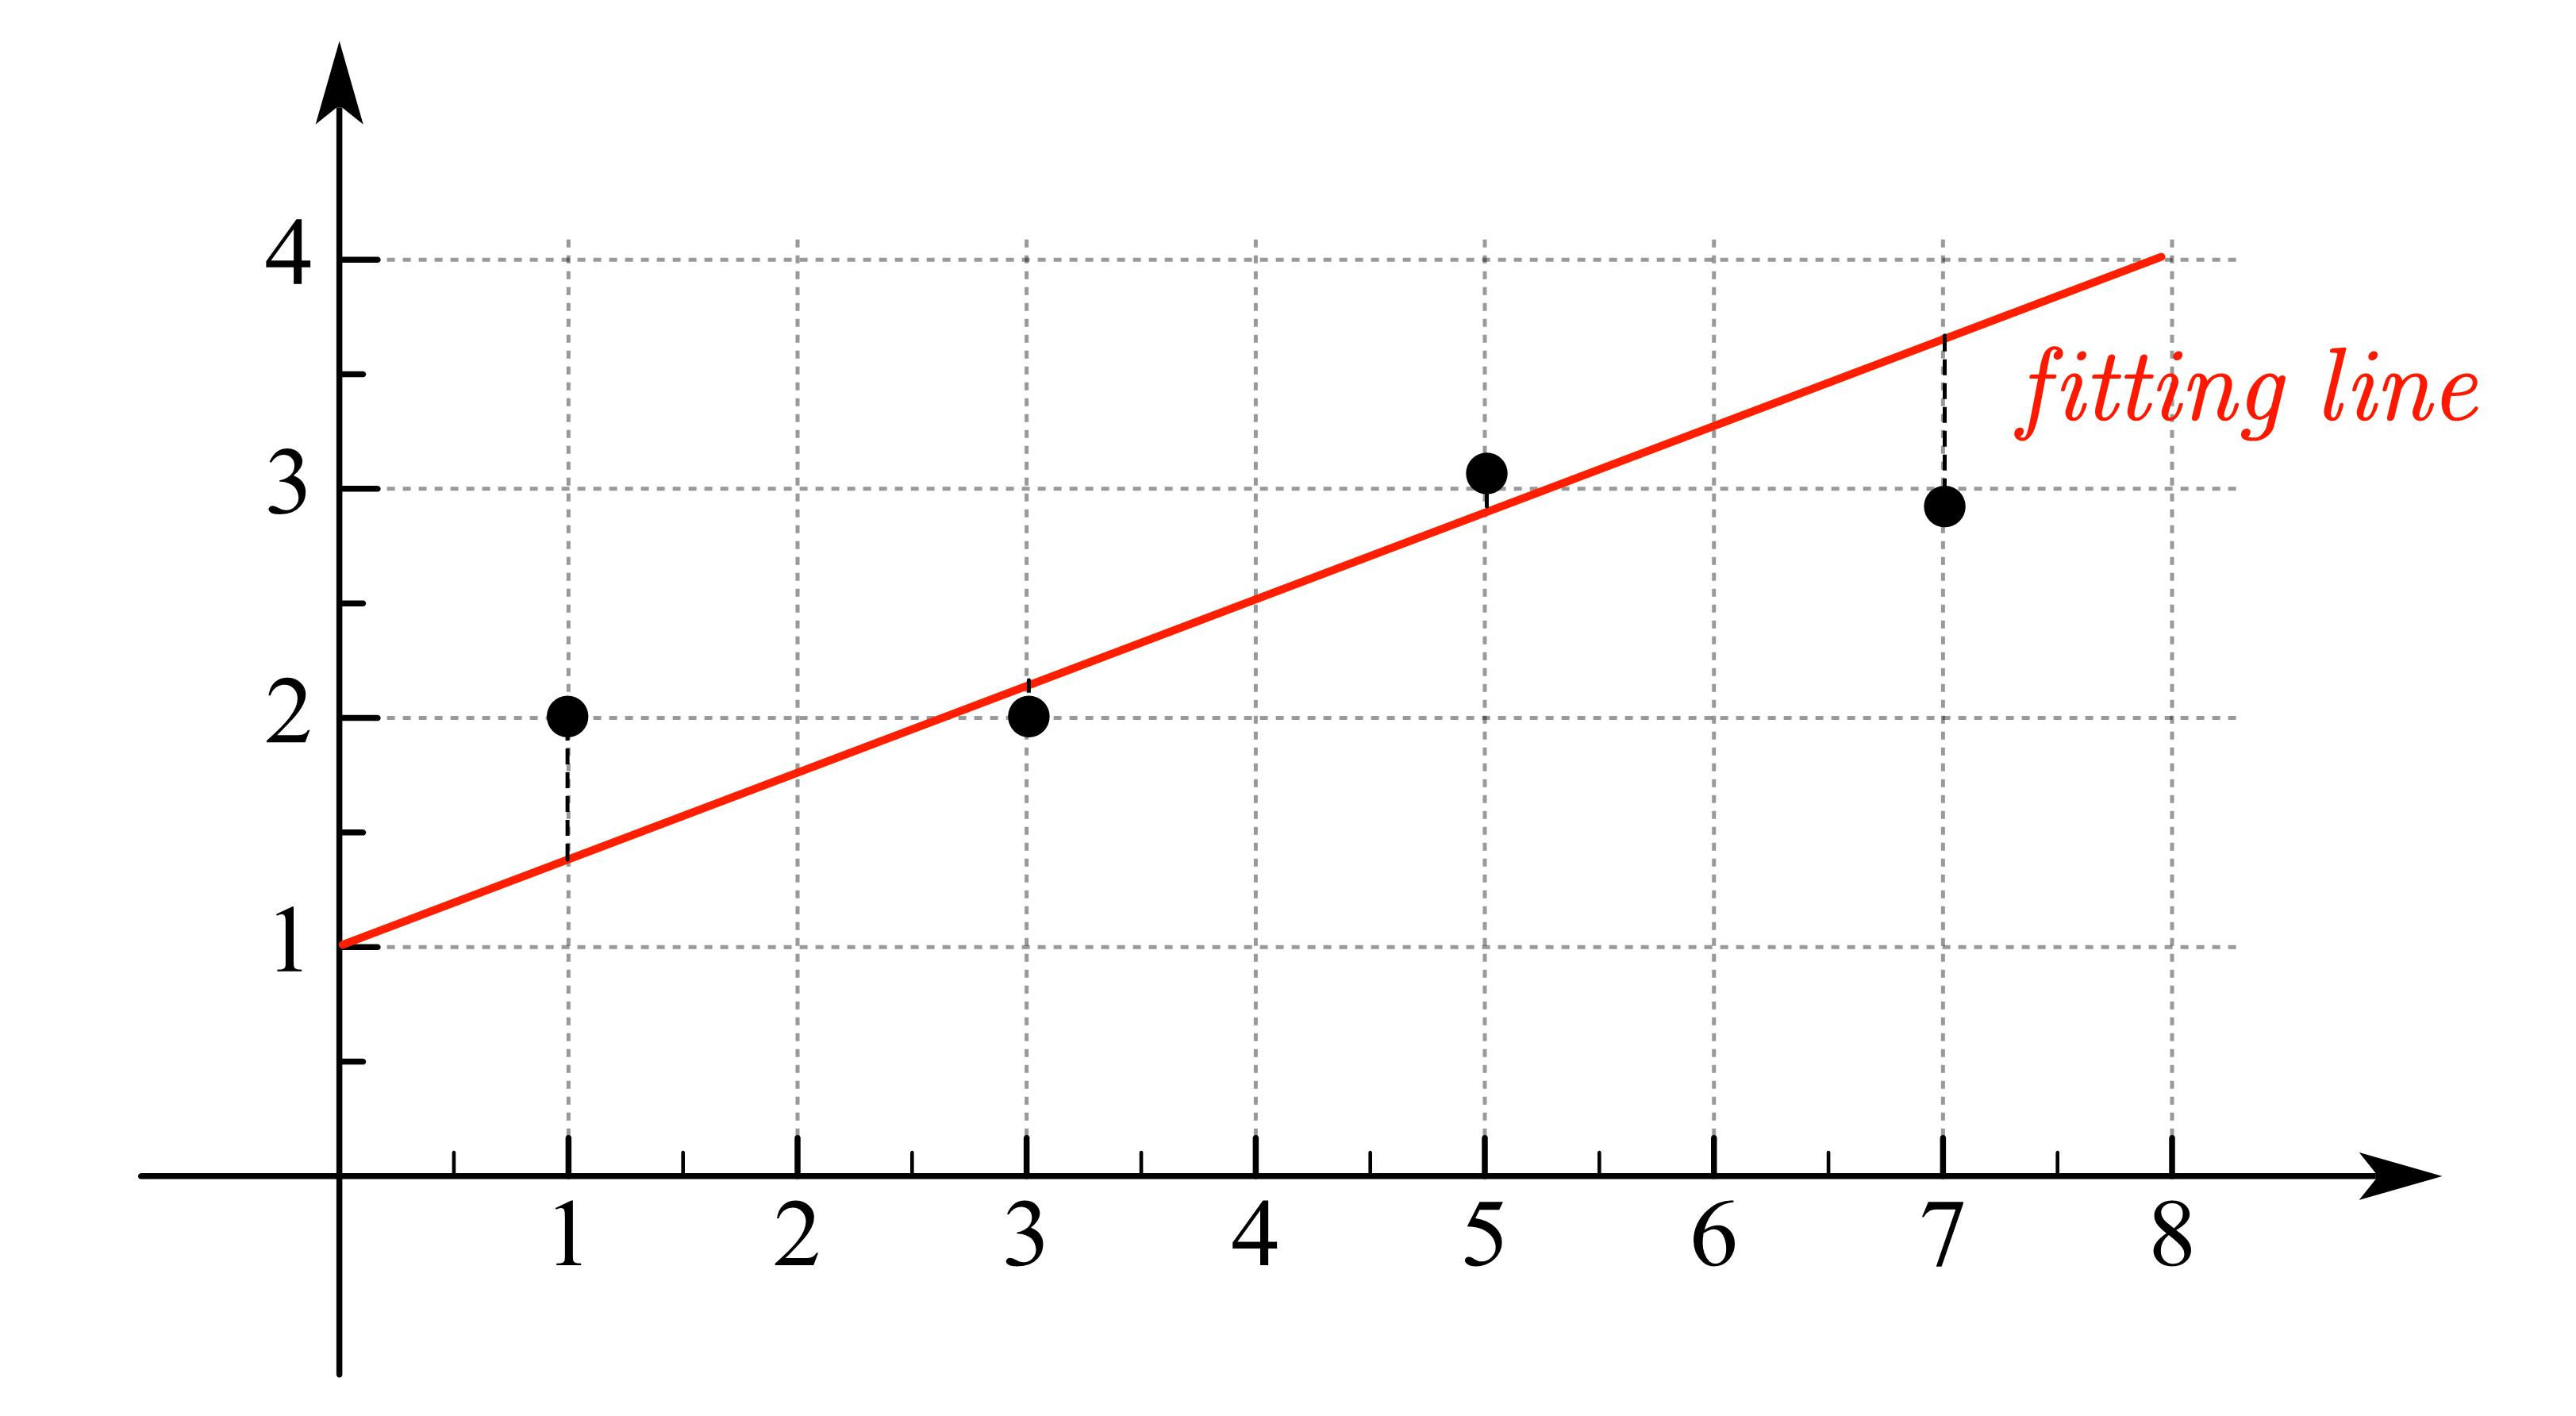
\includegraphics[width=0.62\textwidth]{fitting.jpg}
\end{figure}
We can't find a line to cover all the points, but we can find the line that minimizes the error.
\end{frame}

\begin{frame}{Motivation}
\vspace{3pt}
Take fitting as an example:
\begin{figure}
    \centering
    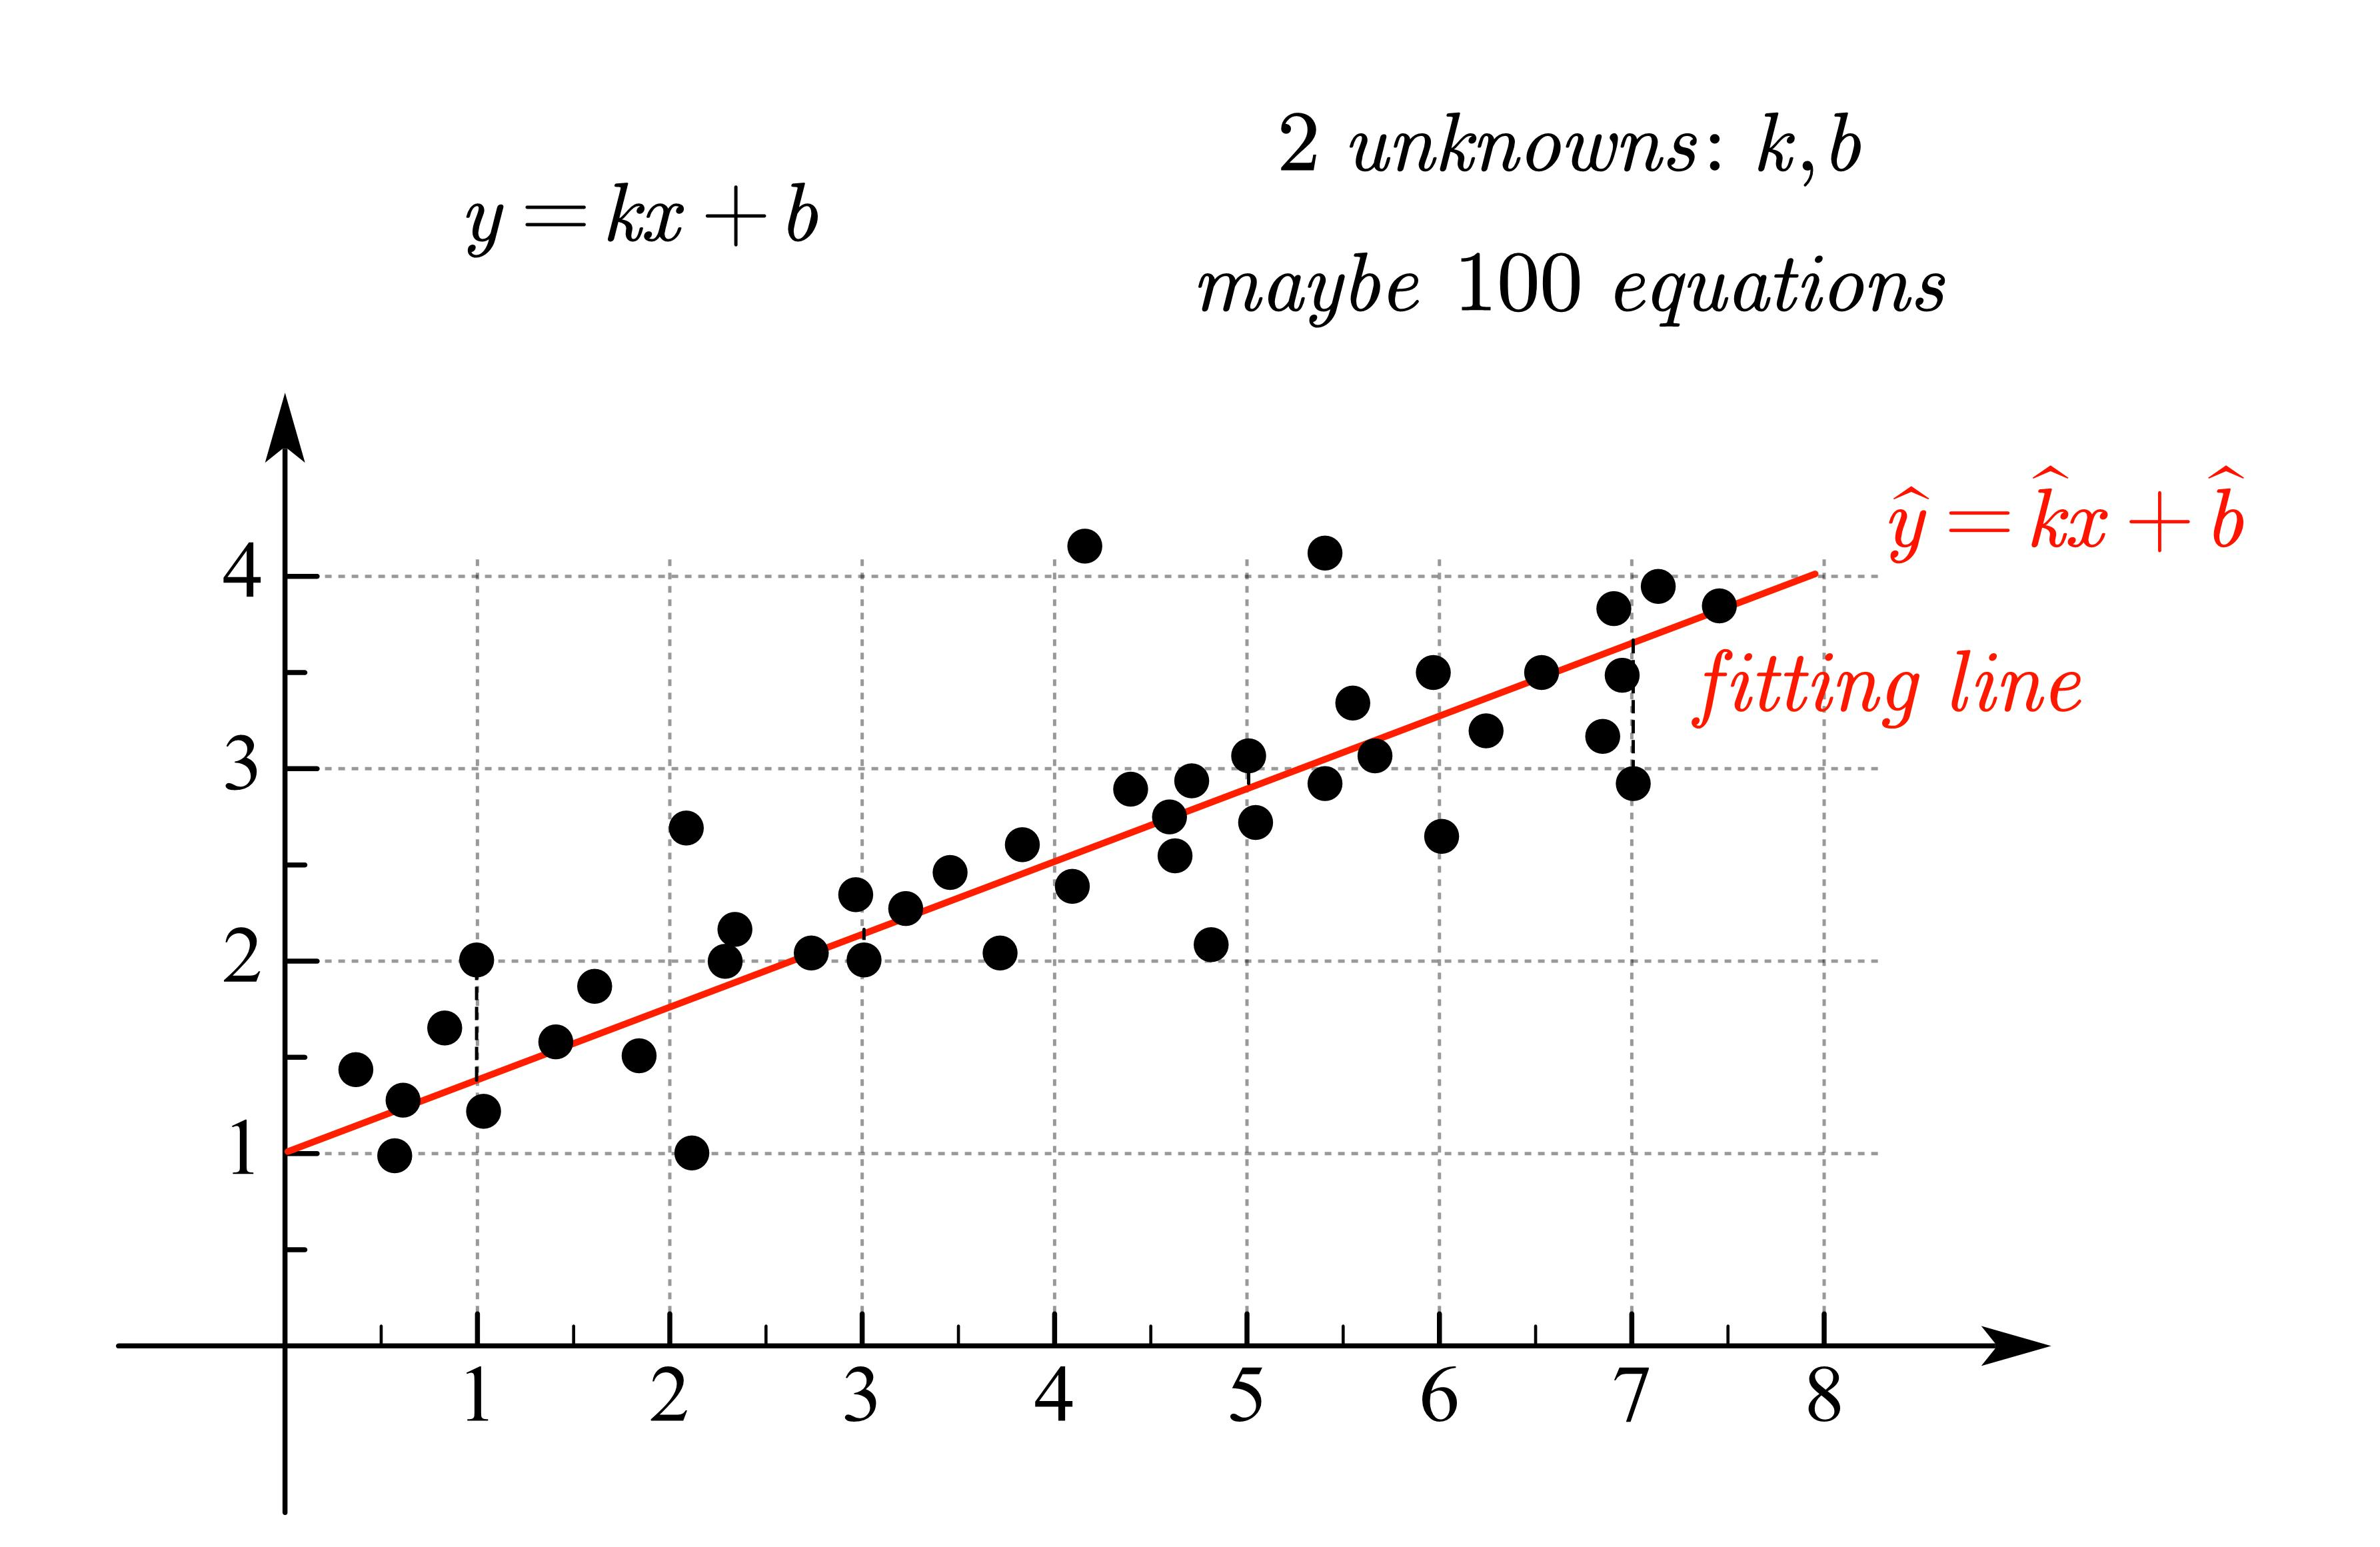
\includegraphics[width=0.75\textwidth]{fitting2.jpg}
\end{figure}

How to find the predicted line? The answer is: least-squares.
\end{frame}

\begin{frame}{Least-Squares}
The core is: find the solution for $Ax=p$ (A is the matrix with $a_1,a_2$ in columns) where $p$ is the projection on $C(A)$, which can definitely gives a unique solution.

\begin{figure}
    \centering
    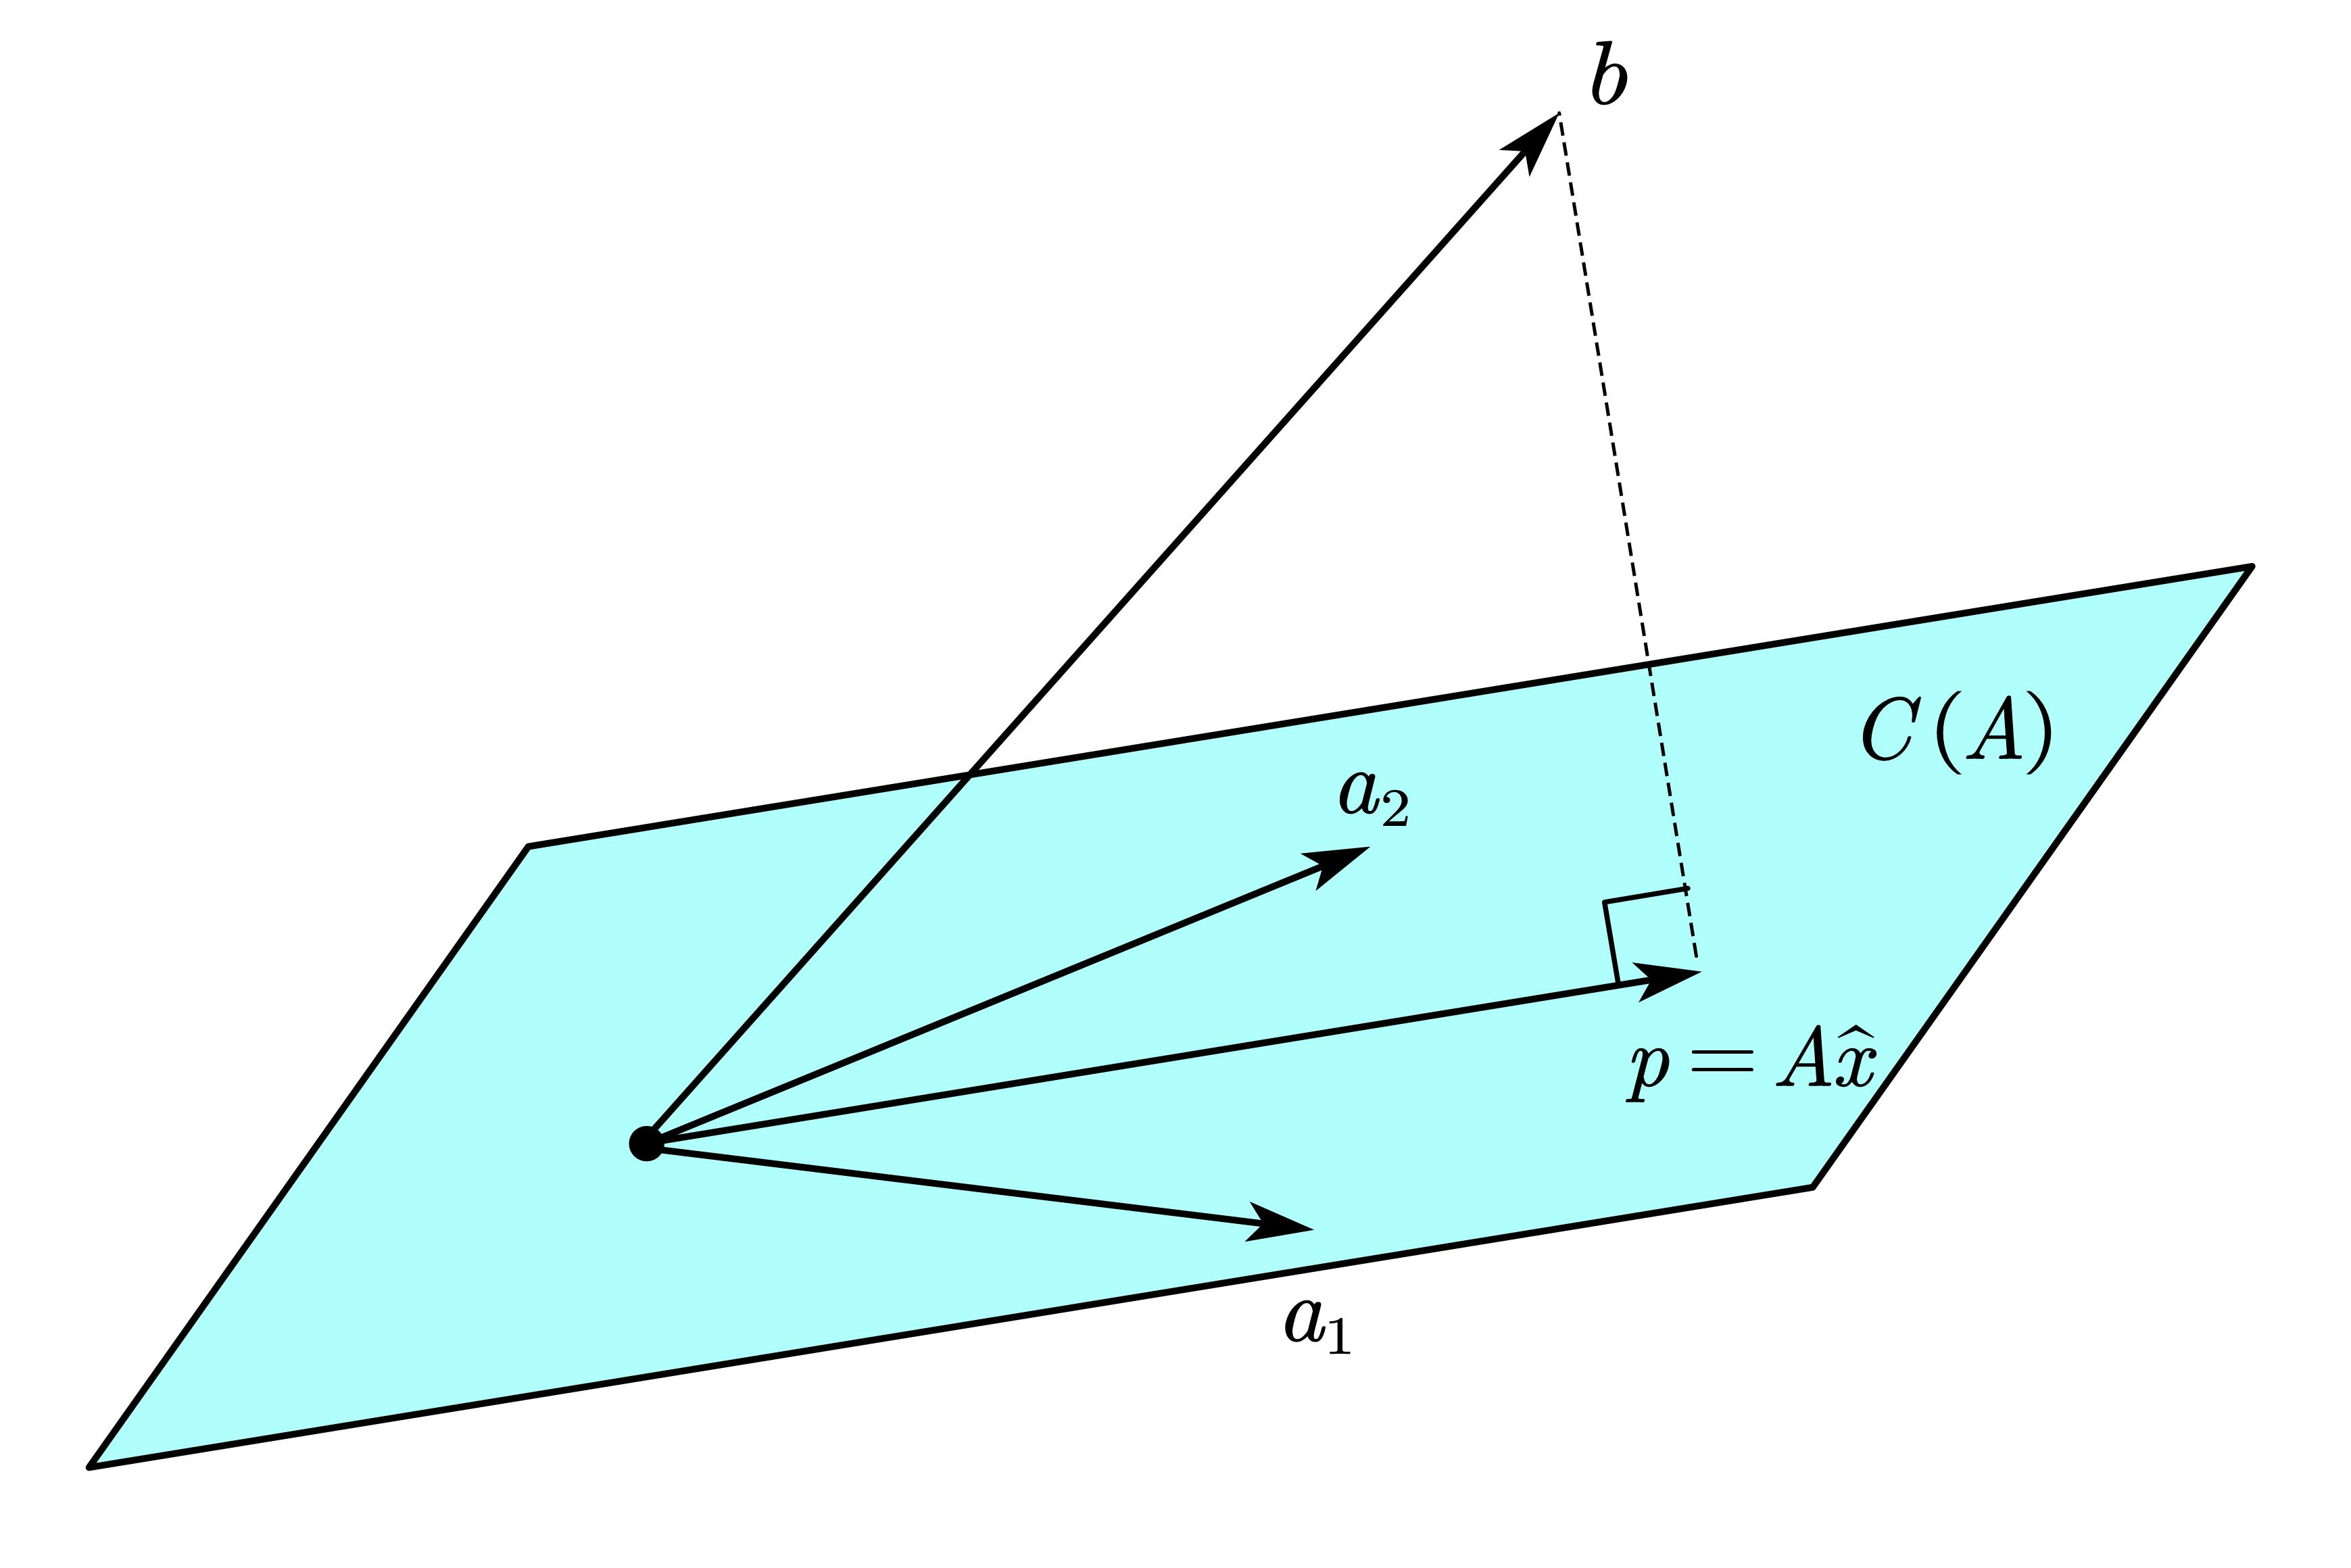
\includegraphics[width=0.5\textwidth]{ls.jpg}
\end{figure}
\begin{equation*}
    {a_1}^T\left( b-A\hat{x} \right) ={a_2}^T\left( b-A\hat{x} \right) =0
\end{equation*}

The error $e=b-p=b-A\hat{x}$ is in the nullspace of $A$, while the projection $p=A\hat{x}$ is in the column space of $A$!
\end{frame}

\begin{frame}{Least-Squares}
Well, we can simplify that equation...
    \begin{equation*}
        {a_1}^T\left( b-A\hat{x} \right) ={a_2}^T\left( b-A\hat{x} \right) =0
    \end{equation*}
\begin{equation*}
    \left[ \begin{array}{c}
        {a_1}^T\\
        {a_2}^T\\
    \end{array} \right] \left( b-A\hat{x} \right) =\left[ \begin{array}{c}
        0\\
        0\\
    \end{array} \right]
\end{equation*}
\begin{equation*}
    A^T\left( b-A\hat{x} \right) =0
\end{equation*}
\begin{equation*}
    A^TA\hat{x} =A^Tb
\end{equation*}

Now, can you tell me why $A^TA\hat{x} =A^Tb$ must be consistent? The reason behind: $Ax=p$ must have solutions.

\vspace{3pt}
Finally, we can get:
\begin{equation*}
    \hat{x} =(A^TA)^{-1}A^Tb
\end{equation*}

That is the least-squares solution, indicating how to combine the columns in $A$ can we get the nearest vector to $b$.
\end{frame}

\begin{frame}{Projection Matrices}
The projection vector in the column space, which is also the nearest vector to $b$ in $C(A)$:
\begin{equation*}
    p=A\hat{x}=A\left( A^TA \right) ^{-1}A^Tb=Pb
\end{equation*}

Now we can have projection matrices onto column space of $A$:
\begin{equation*}
    P=A\left( A^TA \right) ^{-1}A^T
\end{equation*}

Can I take the inverse and simplify the expression further?
\begin{equation*}
    P=A\left( A^TA \right) ^{-1}A^T=AA^{-1}(A^T)^{-1}A^T=I\:???
\end{equation*}

$A$ is not square matrix, $A^{-1}$ doesn't exist.

\vspace{3pt}
Recall that we have introduced projection matrices onto lines:
\begin{equation*}
    P=\frac{\mathbf{aa}^T}{\mathbf{a}^T\mathbf{a}}
\end{equation*}

It is just a special case (1-D case) for projection matrices.
\end{frame}

\section{Interesting Applications of Linear Algebra}
\begin{frame}{Introduction to This Part}
Linear Algebra is definitely a mathematical subject, but it isn't in the Advanced Mathemtics (Calculus) course. That is because linear algebra is the most (not one of the most) useful course in university! The thought and proposed method in linear algebra is useful in all the subject, incluidng chemistry, biology, electrical engineering and computer science...

\vspace{3pt}
We are now studying to use a tool, just like the four elementary computations you learnt in your childhood. With these tools, the complicated concept becomes easier.

\vspace{3pt}
You are not supposed to understand all of the knowledge in this part, but, try to feel the beauty of linear algebra.
\end{frame}

\begin{frame}{Linear Algebra in Chemistry}
How can linear algebra be used in chemistry?

\vspace{3pt}
Recall your chemistry knowledge in your senior high school, try to balance the following chemical reaction equation:
\begin{equation*}
    NO_2+H_2O\rightarrow HNO_3+NO
\end{equation*}

You may use these knowledge:
\begin{itemize}
    \item Mass conservation
    \item Element conservation
\end{itemize}
\end{frame}

\begin{frame}{Linear Algebra in Chemistry}
Here comes Bob, he knows nothing about chemistry, he even doesn't know what $N$ and $O$ represent for. But he is really good at linear algebra, he do the problem by this way:

\vspace{3pt}
Firstly, he set all the codfficients variables $x_1,x_2,x_3,x_4$.
\begin{equation*}
    x_1NO_2+x_2H_2O\rightarrow x_3HNO_3+x_4NO
\end{equation*}

\begin{itemize}
    \item For element $N$: $x_1=x_3+x_4$.
    \item For element $O$: $2x_1+x_2=3x_3+x_4$.
    \item For element $H$: $2x_2=x_3$.
\end{itemize}

\begin{equation*}
    A=\left[ \begin{matrix}
        1&		0&		-1&		-1\\
        2&		1&		-3&		-1\\
        0&		2&		-1&		0\\
    \end{matrix} \right] \rightarrow \left[ \begin{matrix}
        1&		0&		-1&		-1\\
        0&		1&		-1&		1\\
        0&		2&		-1&		0\\
    \end{matrix} \right] \rightarrow \left[ \begin{matrix}
        1&		0&		-1&		-1\\
        0&		1&		-1&		1\\
        0&		0&		1&		-2\\
    \end{matrix} \right]=U
\end{equation*}
\end{frame}

\begin{frame}{Linear Algebra in Chemistry}
\begin{equation*}
    U=\left[ \begin{matrix}
        1&		0&		-1&		-1\\
        0&		1&		-1&		1\\
        0&		0&		1&		-2\\
    \end{matrix} \right] \rightarrow \left[ \begin{matrix}
        1&		0&		0&		-3\\
        0&		1&		0&		-1\\
        0&		0&		1&		-2\\
    \end{matrix} \right] =R
\end{equation*}

He solve the $Ax=0$ system by nullspace matrix, and he gets that:
\begin{equation*}
    x=\left[ \begin{array}{c}
        3\\
        1\\
        2\\
        1\\
    \end{array} \right]
\end{equation*}

The result is
\begin{equation*}
    3NO_2+H_2O= 2HNO_3+NO
\end{equation*}

If you multiply all the coefficients by a constant, the chemical reaction equation is still balanced, but not the simplist.
\end{frame}

\begin{frame}{Linear Algebra in Chemistry}
Not excited? Try this one.
\begin{equation*}
    P_4+CuSO_4+H_2O\rightarrow Cu_3P+H_2SO_4+H_3PO_4
\end{equation*}

\begin{itemize}
    \item For element $P$: $4x_1=x_4+x_6$.
    \item For element $Cu$: $x_2=3x_4$.
    \item For element $S$: $x_2=x_5$.
    \item For element $O$: $4x_2+x_3=4x_5+4x_6$.
    \item For element $H$: $2x_3=2x_5+3x_6$.
\end{itemize}

\begin{equation*}
    \left[ \begin{matrix}
        4&		0&		0&		-1&		0&		-1\\
        0&		1&		0&		-3&		0&		0\\
        0&		1&		0&		0&		-1&		0\\
        0&		4&		1&		0&		-4&		-4\\
        0&		0&		2&		0&		-2&		-3\\
    \end{matrix} \right]
\end{equation*}

Guess the rank of the matrix, give explanations also.
\end{frame}

\begin{frame}{Linear Algebra in Chemistry}
\begin{equation*}
    \left[ \begin{matrix}
        4&		0&		0&		-1&		0&		-1\\
        0&		1&		0&		-3&		0&		0\\
        0&		1&		0&		0&		-1&		0\\
        0&		4&		1&		0&		-4&		-4\\
        0&		0&		2&		0&		-2&		-3\\
    \end{matrix} \right] \rightarrow \left[ \begin{matrix}
        4&		0&		0&		-1&		0&		-1\\
        0&		1&		0&		-3&		0&		0\\
        0&		0&		1&		12&		-4&		-4\\
        0&		0&		0&		3&		-1&		0\\
        0&		0&		0&		0&		-2&		5\\
    \end{matrix} \right]
\end{equation*}

Free variable $x_6$ set to 2, the solution is:
\begin{equation*}
    x=\left[ \begin{matrix}
        11/12&		5&		8&		5/3&		5&		2\\
    \end{matrix} \right] ^T
\end{equation*}

Multiply a constant 12, the solution becomes:
\begin{equation*}
    x=\left[ \begin{matrix}
        11&		60&		96&		20&		60&		24\\
    \end{matrix} \right] ^T
\end{equation*}

So, the final chemical reaction equation is:
\begin{equation*}
    11P_4+60CuSO_4+96H_2O= 20Cu_3P+60H_2SO_4+24H_3PO_4
\end{equation*}
\end{frame}

\begin{frame}{Linear Algebra in Circult Principles}
Three important theorems in circuits:
\begin{itemize}
    \item Ohm's Law: $I=U/R$ for resistors
    \item Kirchhoff's Current Law: $\sum{I}=0$ for each node
    \item Kirchhoff's Voltage Law: $\sum{V}=0$ for each mesh
\end{itemize}

\textbf{Ohm's Law:}
\begin{figure}
    \centering
    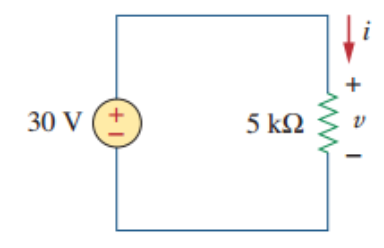
\includegraphics[width=0.35\textwidth]{ohm.png}
\end{figure}

\begin{equation*}
    i=v/R=\frac{30V}{5k\Omega}=6mA
\end{equation*}
\end{frame}

\begin{frame}{Linear Algebra in Circult Principles}
\textbf{Kirchhoff's Current Law (KCL):}
\begin{figure}
    \centering
    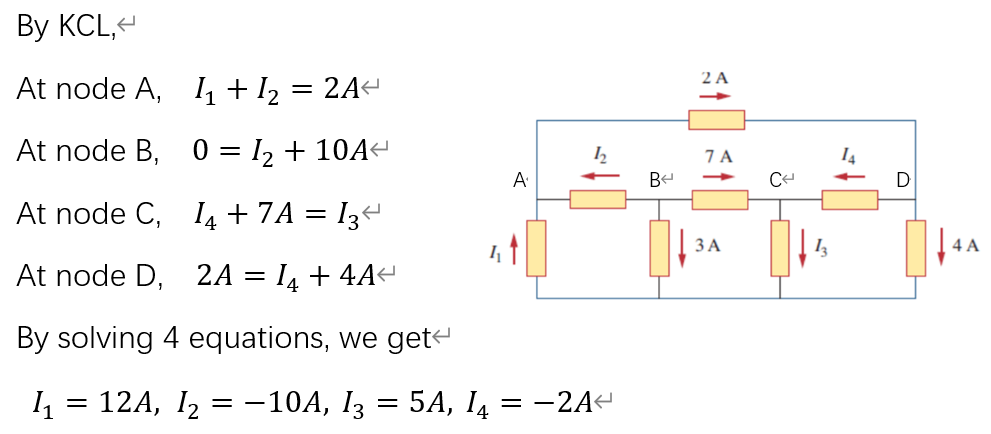
\includegraphics[width=\textwidth]{KCL.png}
\end{figure}
\end{frame}


\begin{frame}{Linear Algebra in Circult Principles}
    \textbf{Kirchhoff's Voltage Law (KVL):}
\begin{figure}
    \centering
    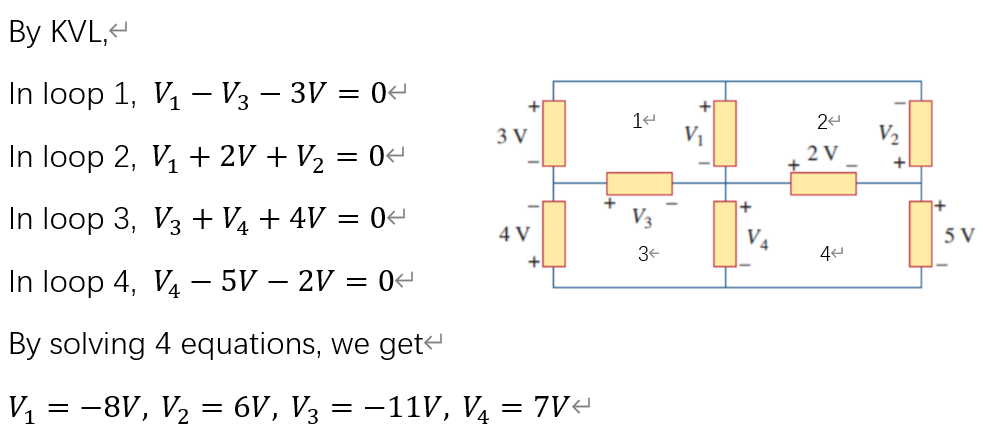
\includegraphics[width=\textwidth]{KVL.png}
\end{figure}
\end{frame}

\begin{frame}{Linear Algebra in Circult Principles}
Seems to be easy... But for complicated circuit, can you figure out the whole state of it?

\begin{figure}
    \centering
    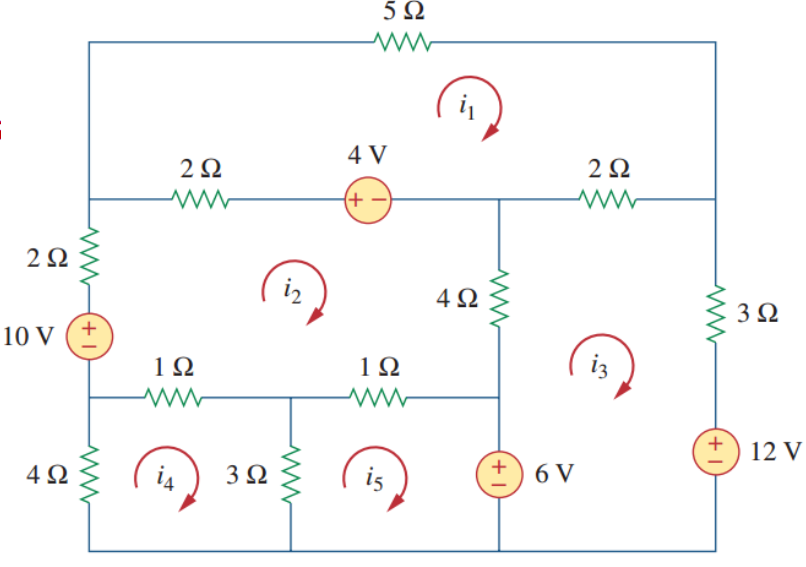
\includegraphics[width=0.6\textwidth]{example.png}
\end{figure}

Our method is: find the mesh current $i_1, i_2, i_3, i_4, i_5$.
\end{frame}

\begin{frame}{Linear Algebra in Circult Principles}
The essence: Solve $Ax=b$ linear system!
\begin{figure}
    \centering
    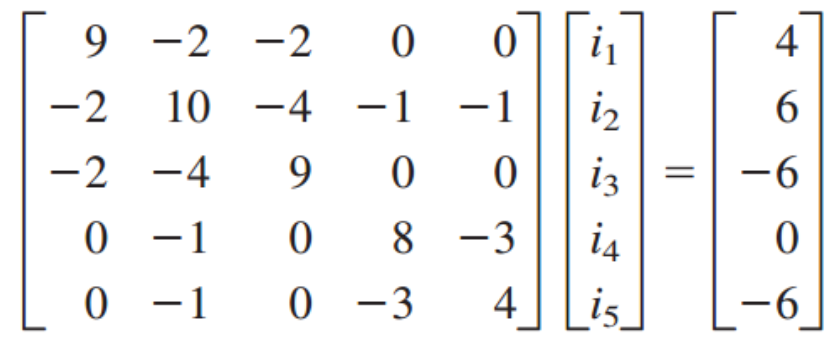
\includegraphics[width=0.6\textwidth]{eq.png}
\end{figure}

Every row is a KVL equation for a mesh.

\vspace{3pt}
If there is no voltage source, then the equation system becomes $Ax=0$, the mesh currents are definitely all zero (that is to say the matrix is of full rank because all the meshes are independent, no repeat meshes occur)!

\vspace{3pt}
The result will be
\begin{equation*}
    i_1=0.283A,i_2=0.211A,i_3=-0.488A,i_4=-0.718A,i_5=-1.986A
\end{equation*}

\end{frame}



\begin{frame}{Linear Algebra in Computer Vision}
Computer Vision is a great subject in artificial intelligence. Let's have a brief introduction about how our images are like in the computer view.

\vspace{3pt}
In a computer, how does it read or store an image?

\begin{figure}
    \centering
    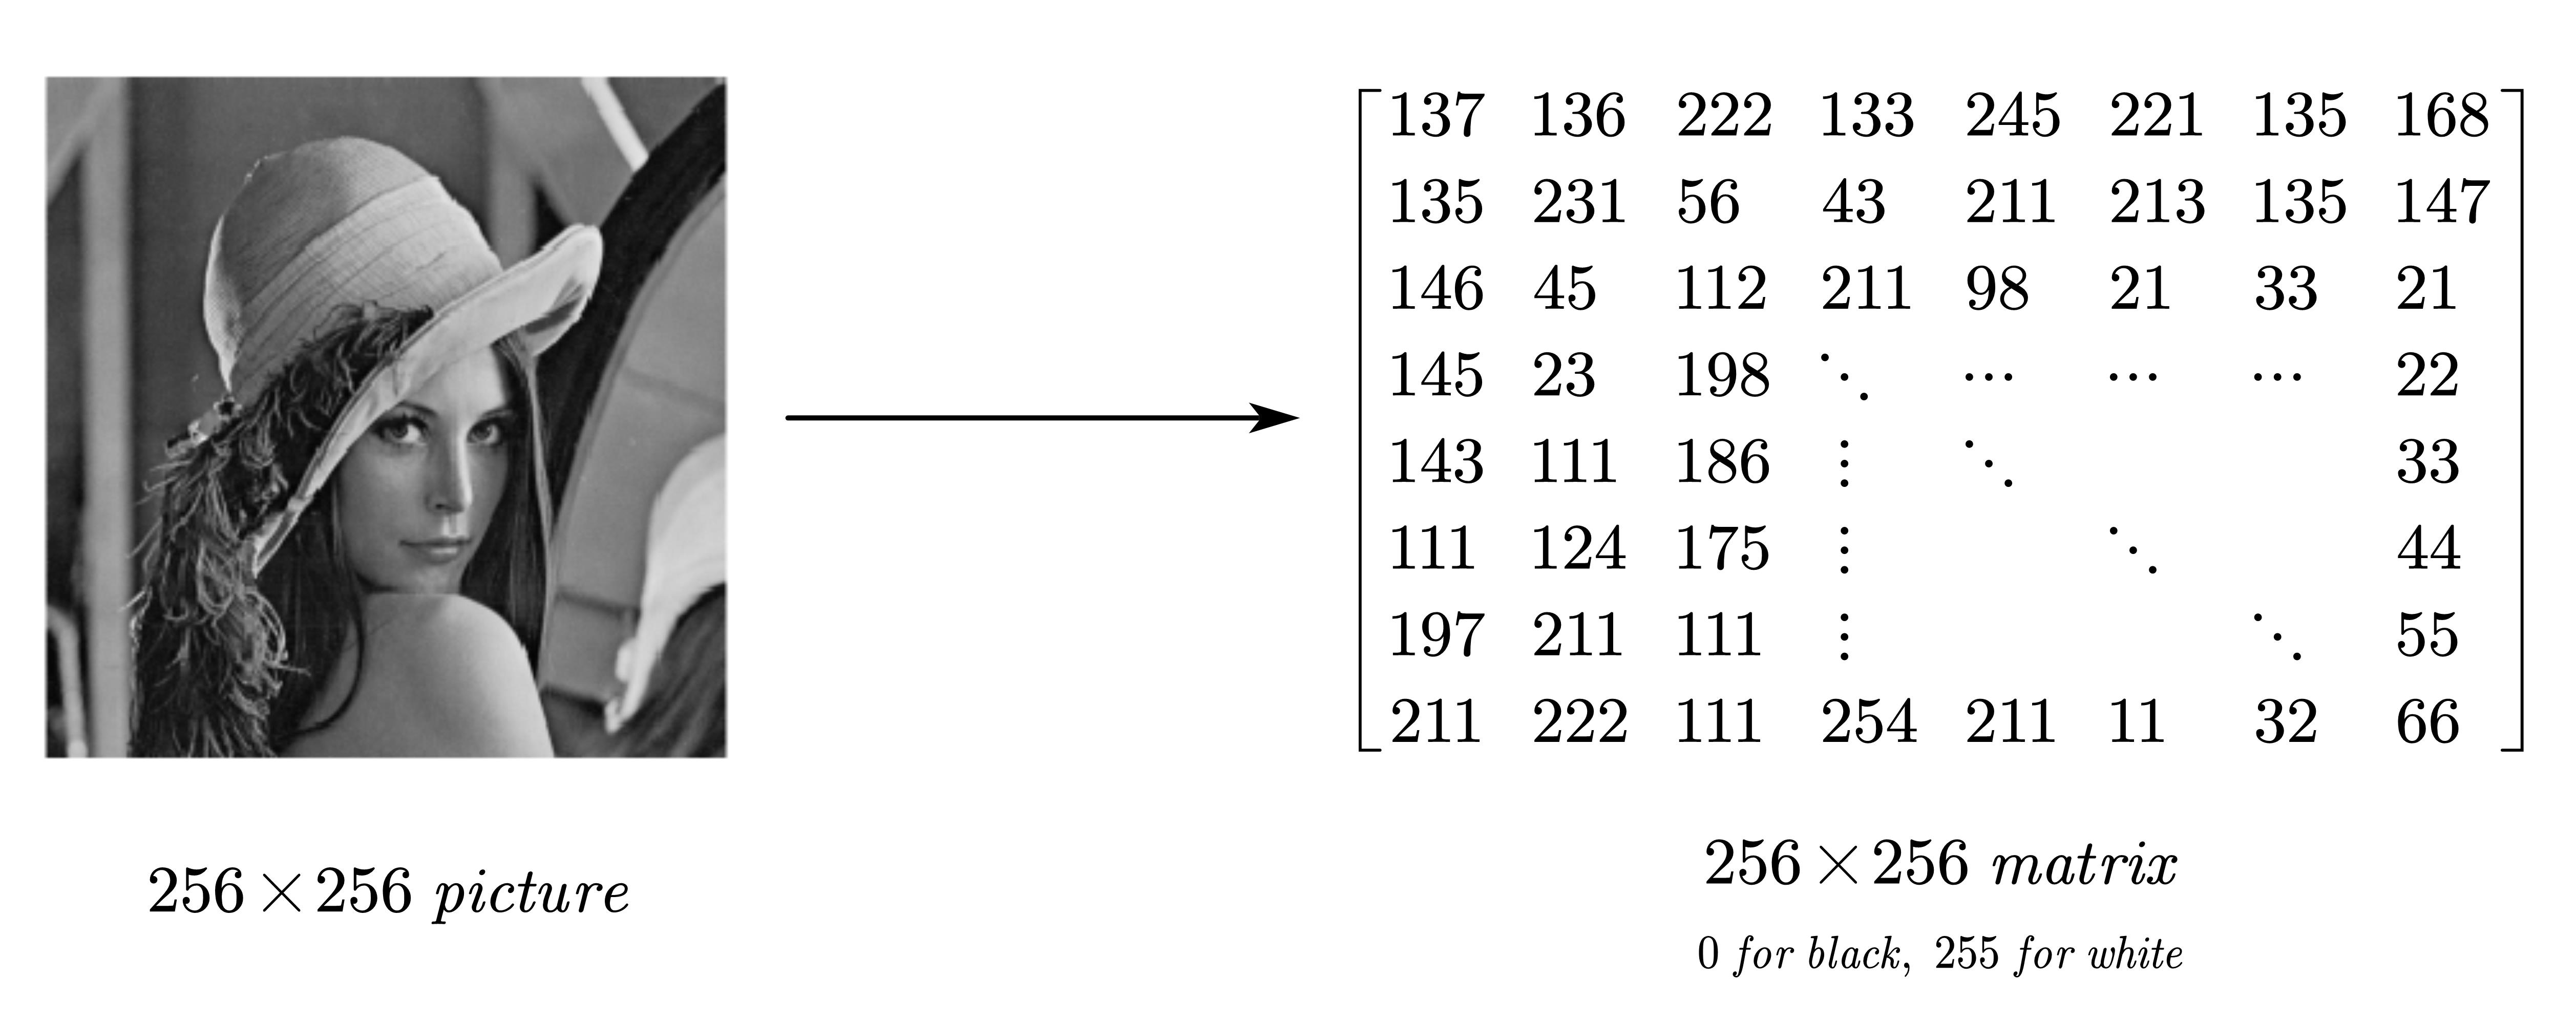
\includegraphics[width=0.98\textwidth]{lena.jpg}
\end{figure}
\vspace{-8pt}
It is a natural matrix! If a picture is colorful, then we may have 3 $256\times 256$ matrices for ${\color{red} R}, {\color[RGB]{0, 255, 0} G}, {\color{blue} B}$ respectively.
\end{frame}

\begin{frame}{Linear Algebra in Computer Vision}
A new operation: convolution.

\begin{figure}
    \centering
    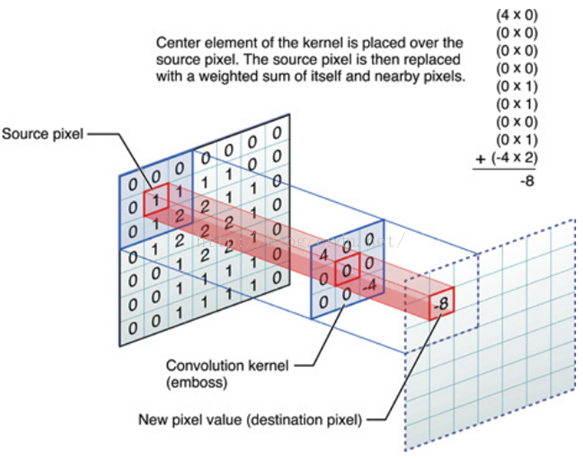
\includegraphics[width=0.6\textwidth]{conv.png}
\end{figure}

Now, let's see what will happen for different convolution kernal.
\end{frame}

\begin{frame}{Linear Algebra in Computer Vision}
    \begin{itemize}
        \item Identity:
        \begin{figure}
            \centering
            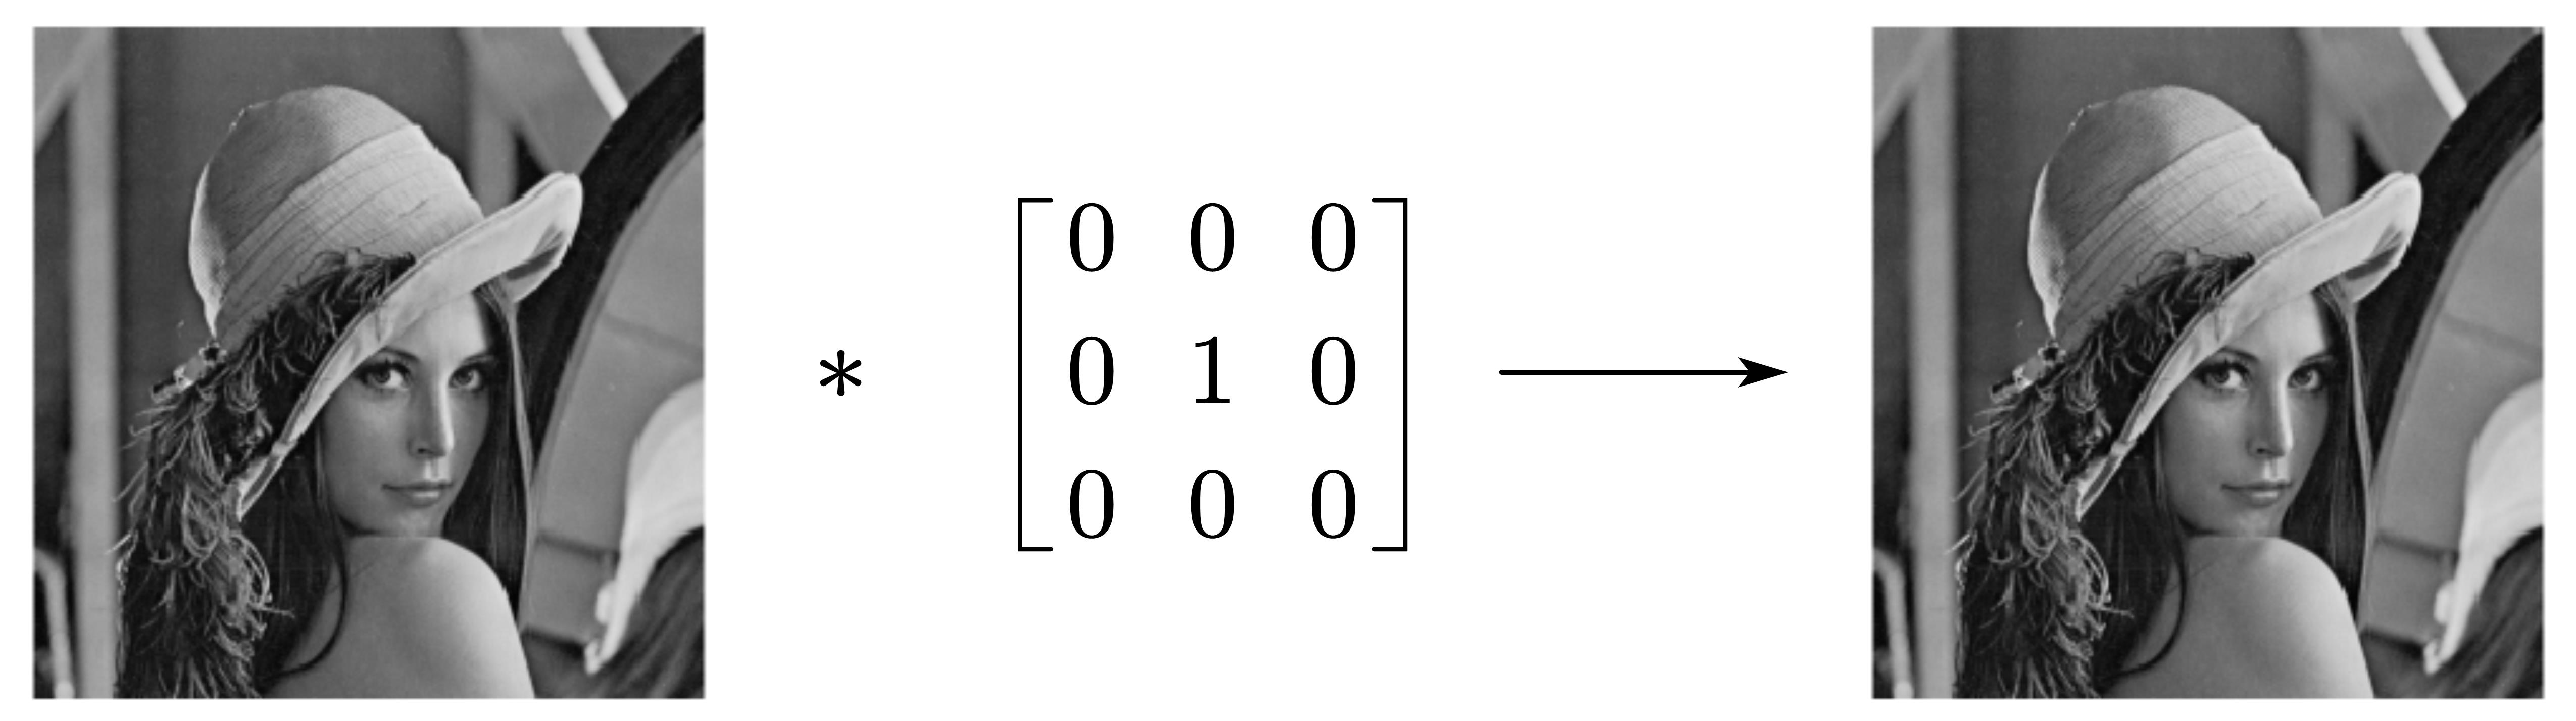
\includegraphics[width=0.8\textwidth]{lena1.jpg}
        \end{figure}
        \item Sharpen:
        \begin{figure}
            \centering
            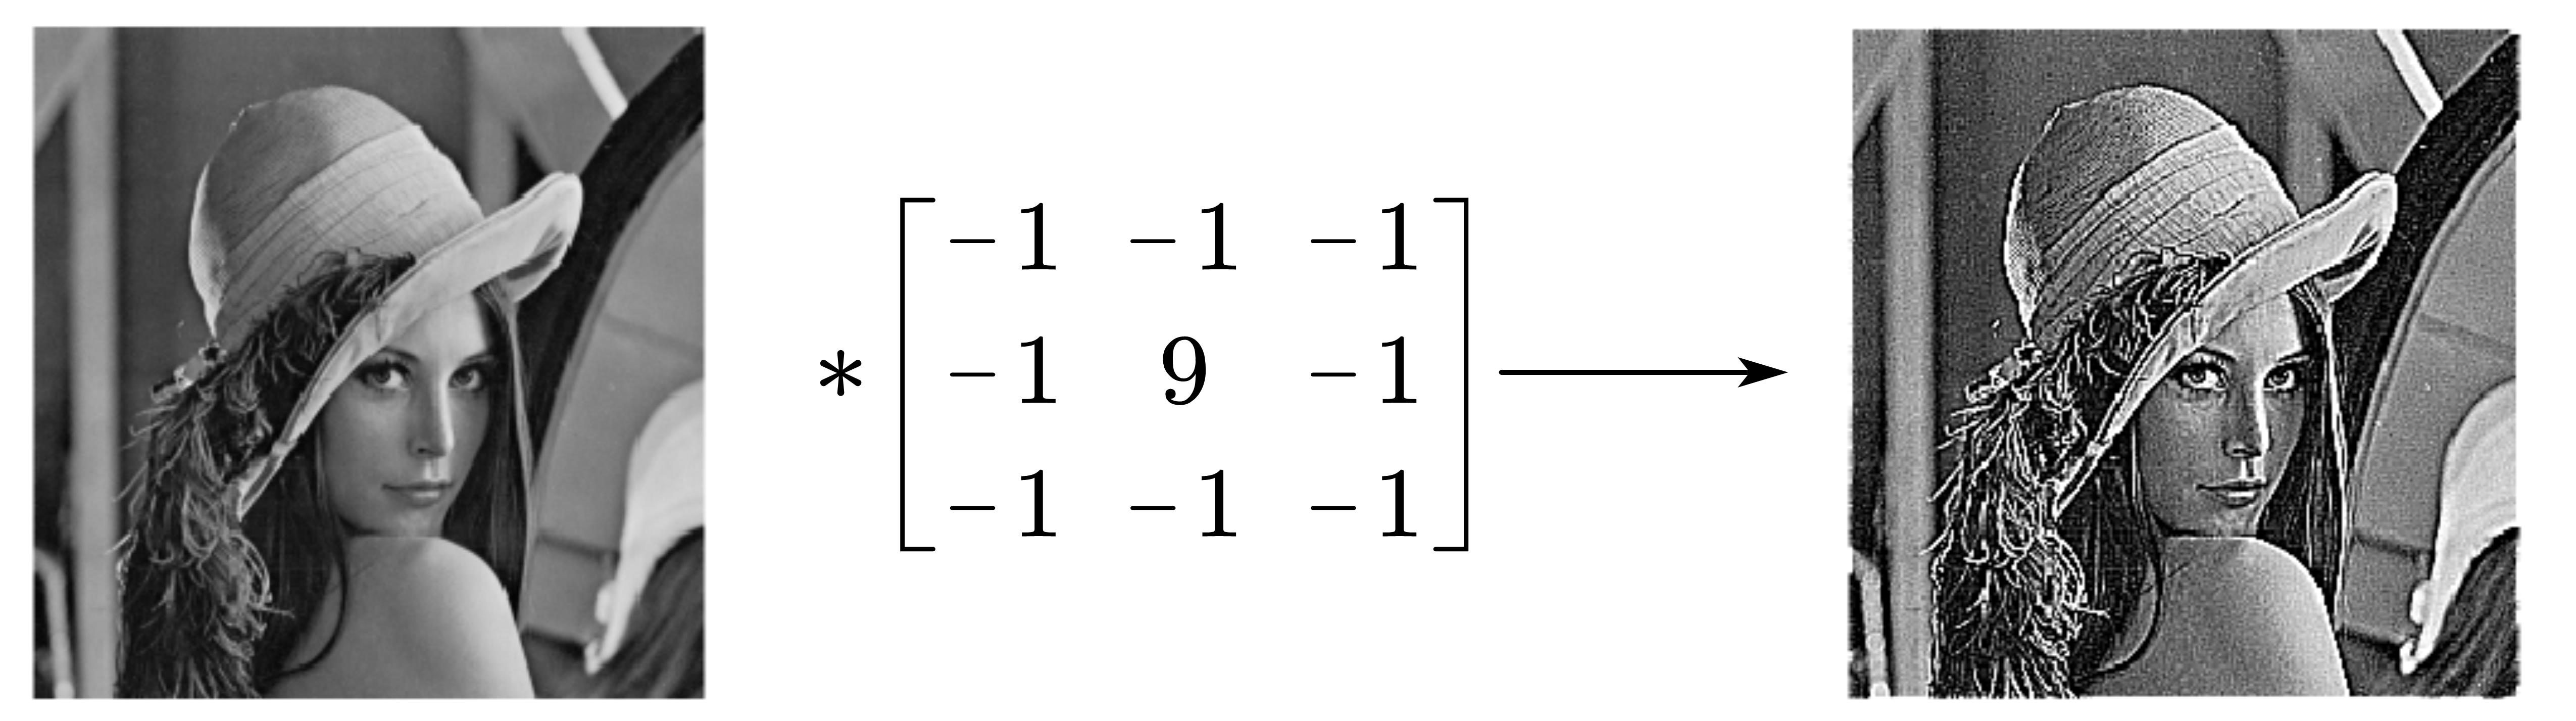
\includegraphics[width=0.8\textwidth]{lena2.jpg}
        \end{figure}
    \end{itemize}

\end{frame}
\end{document}